\documentclass[12pt,a4paper]{article}
\usepackage{iftex}
\ifXeTeX
  \usepackage{fontspec}
  \IfFontExistsTF{Times New Roman}{\setmainfont{Times New Roman}}{\setmainfont{TeX Gyre Termes}}
\else\ifLuaTeX
  \usepackage{fontspec}
  \IfFontExistsTF{Times New Roman}{\setmainfont{Times New Roman}}{\setmainfont{TeX Gyre Termes}}
\else
  \usepackage[T1]{fontenc}\usepackage[utf8]{inputenc}\usepackage{mathptmx}
\fi\fi
\usepackage{textcomp}
\usepackage[margin=2.5cm]{geometry}
\usepackage{graphicx,booktabs,tabularx,xltabular,enumitem,xcolor,caption,amsmath}
\usepackage[hidelinks]{hyperref}\urlstyle{same}
\definecolor{boxbg}{HTML}{F3EEE4}
\captionsetup{labelformat=empty,justification=raggedright,singlelinecheck=false,skip=4pt}
\setlength{\parindent}{0pt}\setlength{\parskip}{6pt}
\renewcommand{\arraystretch}{1.25}
\usepackage{titlesec}
\titleformat{\section}{\large\bfseries}{}{0pt}{}
\titleformat{\subsection}{\normalsize\bfseries}{}{0pt}{}
\titlespacing*{\section}{0pt}{14pt}{4pt}
\titlespacing*{\subsection}{0pt}{10pt}{2pt}
\usepackage{fancyhdr}\pagestyle{fancy}\fancyhf{}\renewcommand{\headrulewidth}{0pt}
\fancyfoot[C]{\small\thepage}\fancyhead[R]{\small\textsc{T-Minus Markets}}
\begin{document}
{\raggedright{\LARGE\bfseries Rocket Launch Failures and Equity-Market Spillovers: Evidence from Publicly Listed Launch Providers\par}\vspace{6pt}{\large A T-Minus Markets case study of stock market reactions to orbital launch failures, 2000 to 2026.\par}\vspace{8pt}{\normalsize Nahian Ibnat \textperiodcentered{} Nov 2026\par}{\small Interactive version: \url{https://nahianibnat-2000.github.io/T-Minus-Market/}\par}}
\vspace{6pt}
\begin{abstract}
\noindent This paper asks how equity markets react when an orbital launch fails, both for the company that built the rocket and for its publicly listed competitors. Using 138 orbital launch failures from 2000 to 2026 (GCAT) and a market-model event study with a prespecified test, it finds that in the 4 failures with a listed maker (2 firms) the maker lost between 8.8\% and 16.3\% of market value over two trading days, each case with a 95\% interval excluding zero. Across 24 failures with listed competitors (42 stock reactions, 3 firms, 22 independent events), the average two-day cumulative abnormal return is +0.28\% (95\% cluster-robust interval \textminus{}1.62\% to +2.18\%; Boehmer-Musumeci-Poulsen test with Kolari-Pynnönen adjustment, p = 0.40). The evidence therefore establishes neither systematic contagion nor systematic competitive gains among these firms, and it does not show the effect is negligible: average effects of about 2.7\% in either direction would usually go undetected. The sign of the estimate changes with how events and firms are weighted, and every independent event involves Avio SpA. The study is a small-sample case study of listed firms, not an estimate for the launch industry as a whole.

\textbf{Keywords:} event study; industry spillovers; contagion; competitive effects; launch failures. \textbf{JEL:} G14, L13.
\end{abstract}

\section*{1. Introduction}
When a rocket fails, the company that built it loses hardware, often a customer's satellite, and usually months of flights while the cause is investigated. Its competitors face a less obvious outcome. Investors may read the failure as a reminder that spaceflight is risky for every provider, which lowers rivals' values (contagion), or they may expect customers to move to providers whose rockets work, which raises them (competitive gain). The two channels push in opposite directions, so the net reaction of rivals is an empirical question.

This paper measures both reactions with a short-window event study. Launch failures suit the method: they are sudden, public, precisely timed, and unrelated to the rivals' own decisions. The confirmatory hypothesis (H2) is that the average two-day abnormal return of listed rivals is zero. All rules were fixed in a written plan committed to the project repository before any abnormal return was computed.

The answer is limited by the sample. Only 3 listed launch firms qualify as direct rivals at the time of a failure, so the study observes 22 independent rival events, every one of which involves Avio SpA. The average reaction is not distinguishable from zero, but the interval is wide enough to contain economically meaningful losses and gains. The contribution is therefore a carefully documented, reproducible estimate with honest uncertainty, rather than a general claim about the launch industry.

Section 2 describes the industry; section 3 relates the study to earlier work; sections 4 and 5 describe data and methods; sections 6 to 8 report results, robustness and confounding news; sections 9 to 11 discuss, list limitations and conclude.

\section*{2. Institutional background}
\textbf{A concentrated market.} Orbital launch is supplied by a small number of providers, many of them state agencies, state-owned firms or privately held companies. Launch contracts are usually signed years ahead, and a satellite is designed for a particular rocket, so customers cannot switch providers quickly. This limits how much business a rival can win in the days after a failure.

\textbf{Reliability.} New rockets fail more often than mature ones, and a failure normally grounds the vehicle until an investigation is complete. For the maker, the loss includes the hardware, possible penalties or re-flights, delay of other launches and reputation.

\textbf{Ownership and listing.} Few launch companies have been publicly traded with launch as a major business. Large aerospace groups that build rockets are diversified, so a launch failure is a small part of their value; the plan therefore counts them only when launch is a major part of the business. The listed pure-play or launch-heavy firms in the sample listed only in the last decade, so the sample of listed rival events starts late. SpaceX listed in June 2026 and has too little price history to enter.

\textbf{Disclosure.} Most launches are broadcast live, so a failure becomes public at launch time. Where a failure is confirmed later, the first public company statement dates the event.

\section*{3. Related literature}
\textbf{Event-study method.} The design follows MacKinlay (1997) and Brown and Warner (1985) for daily returns. The standardized test of Boehmer, Musumeci and Poulsen (1991) allows the event to raise return variance, and Kolari and Pynnönen (2010) show that cross-sectional correlation among event-day abnormal returns biases standard tests, and propose the adjustment used here. Corrado (1989) supplies a rank-based alternative.

\textbf{Contagion and competitive effects.} Lang and Stulz (1992) find that bankruptcy announcements lower the value of a portfolio of competitors by about 1\% on average, so contagion dominates in that setting. Bosch, Eckard and Singal (1998) study rival airlines after air crashes, testing whether customers switch carriers or fly less.

\textbf{Disasters and investor sentiment.} Kaplanski and Levy (2010) report market-wide losses after aviation disasters that reverse within days, consistent with sentiment rather than fundamentals. For spaceflight, Blose et al. (1996) and Maloney and Mulherin (2003) study the Challenger disaster: NASA contractors fell together on the day, and within days the market singled out the firm whose component failed.

\textbf{Launch markets.} Abramov and Kiang (2015) study how launch delays and failures affect satellite operators, the launch customers. Do et al. (2023) show that US satellite launch days draw investor attention away from firm-specific news. This paper studies a different group, the failed provider's listed competitors, over a multi-year sample.

\section*{4. Data and sample construction}
\textbf{Launch records.} Every orbital launch attempt comes from GCAT (McDowell). A launch is a failure when its GCAT success score is below 0.75; pad explosions before launch are kept separately. Launch times come from GCAT's launch date field; where the company confirmed a failure later, the documented disclosure time is used and its confidence is recorded.

\textbf{Firms.} Each failure is linked by hand, point in time, to its maker if listed and to listed rivals. A Tier 1 rival is listed, has launch as a pure-play or major business, sells a rocket of the same size class to the same customer market, and has flown that rocket in the previous 730 days. Firm-map rows used in tests are verified against filings or exchange notices.

\textbf{Prices.} Daily adjusted closes from Yahoo Finance, used locally only; benchmarks are each firm's home market index. Prices from before a firm's real listing (a pre-merger shell) are dropped. Only derived statistics are published.

\textbf{Event dates and clusters.} Day 0 (T0) is the first trading session at or after the failure became public, on the stock's own exchange calendar. Failures less than 5 trading days apart that share a firm form one cluster.

\begin{figure}[htbp]\centering
\caption*{\textbf{Figure 1.} Sample construction}
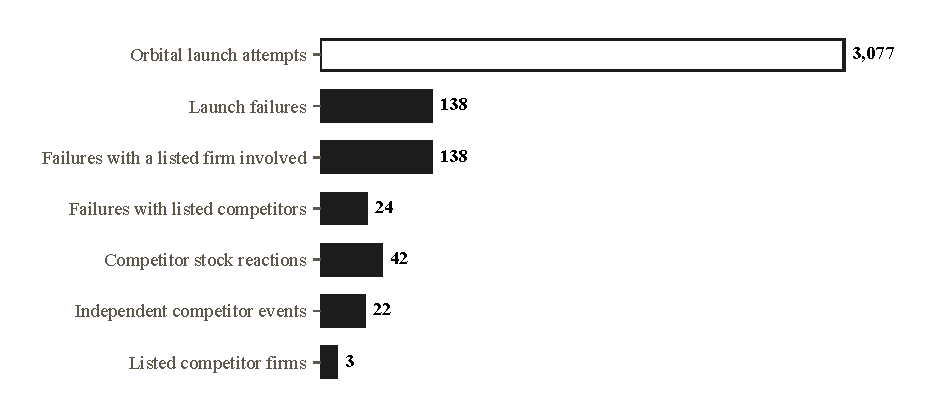
\includegraphics[width=\textwidth]{fig-funnel.pdf}
\par\vspace{2pt}{\footnotesize Bar length on a square-root scale. Counts come from the pipeline's interim files and exported data.}
\end{figure}

\begin{figure}[htbp]\centering
\caption*{\textbf{Figure 2.} Orbital launch failures per year}
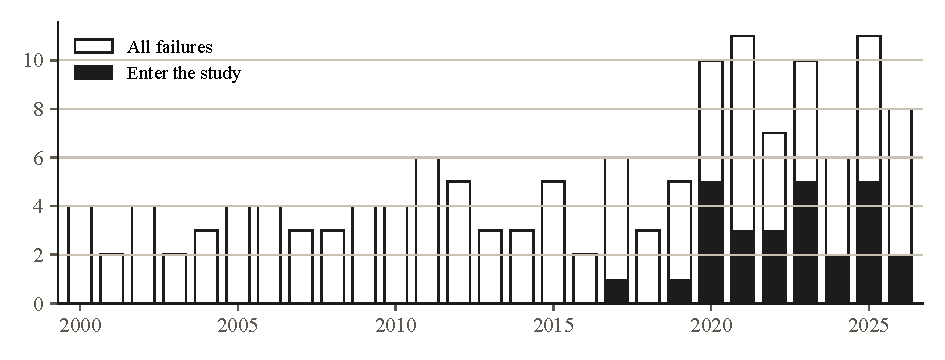
\includegraphics[width=\textwidth]{fig-years.pdf}
\par\vspace{2pt}{\footnotesize Outline: all orbital launch failures, 2000 to 2026. Filled: failures that enter the study.}
\end{figure}

\par\noindent\begin{minipage}{\textwidth}
\textbf{Table 1.} Rival reactions by firm, CAR T0 to T+1

{\small\setlength{\tabcolsep}{4pt}\begin{tabularx}{\textwidth}{Xllllll}
\toprule
\textbf{Firm} & \textbf{Ticker} & \textbf{Reactions} & \textbf{Clusters} & \textbf{Mean} & \textbf{Median} & \textbf{Range} \\
\midrule
Avio SpA & AVIO.MI & 24 & 22 & +0.60\% & +0.28\% & \textminus{}7.3\% to +14.5\% \\
Rocket Lab & RKLB & 15 & 14 & +0.79\% & +0.43\% & \textminus{}7.4\% to +25.3\% \\
Firefly Aerospace & FLY & 3 & 3 & \textminus{}4.86\% & \textminus{}6.07\% & \textminus{}7.0\% to \textminus{}1.5\% \\
\textbf{All} &  & 42 & 22 & +0.28\% & +0.28\% & \textminus{}7.4\% to +25.3\% \\
\bottomrule
\end{tabularx}}
\vspace{6pt}

Clusters: independent events in which the firm appears; 22 in total.

\end{minipage}\par\vspace{4pt}

\begin{figure}[htbp]\centering
\caption*{\textbf{Figure 3.} Which rival is present in each independent event}
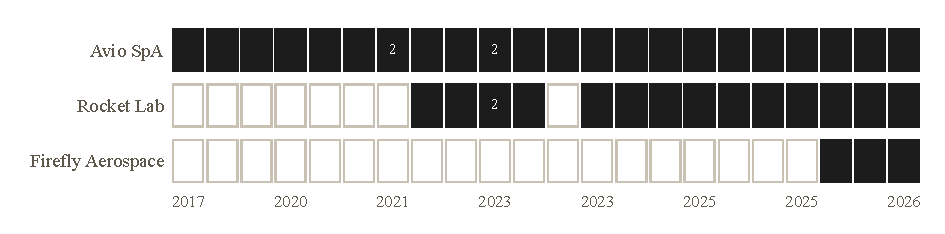
\includegraphics[width=\textwidth]{fig-exposure.pdf}
\par\vspace{2pt}{\footnotesize Columns: independent events in date order. Filled: the firm is a rival in that event; a number means it appears more than once (two close failures).}
\end{figure}

\section*{5. Empirical methodology}
For each stock and failure a market model is estimated by ordinary least squares on trading days 250 to 30 before day 0 (at least 100 returns; with 30 to 99 returns a market-adjusted model with α = 0 and β = 1 is used and flagged):

\begin{equation}
R_{it} = \alpha_i + \beta_i R_{mt} + \varepsilon_{it}
\end{equation}

Abnormal returns and cumulative abnormal returns over an event window [τ1, τ2] are

\begin{equation}
AR_{it} = R_{it} - (\hat\alpha_i + \hat\beta_i R_{mt}), \qquad CAR_i(\tau_1,\tau_2) = \sum_{t=\tau_1}^{\tau_2} AR_{it}
\end{equation}

Returns are simple, and CARs are sums of simple abnormal returns. The variance of each CAR includes the prediction error of the estimated model (Campbell, Lo and MacKinlay, 1997), where \emph{L} is the window length, \emph{T} the number of estimation days, \emph{W} the event window and \emph{E} the estimation window:

\begin{equation}
\mathrm{Var}(CAR_i) = \hat\sigma_i^2\left[L + \frac{L^2}{T} + \frac{\left(\sum_{t\in W}(R_{mt}-\bar R_m)\right)^2}{\sum_{t\in E}(R_{mt}-\bar R_m)^2}\right]
\end{equation}

The confirmatory test is the standardized test of Boehmer, Musumeci and Poulsen (1991), which uses the cross-sectional spread of standardized CARs and so allows the failure to raise variance:

\begin{equation}
SCAR_i = \frac{CAR_i}{\sqrt{\mathrm{Var}(CAR_i)}}, \qquad t_{BMP} = \frac{\sqrt{N}\,\overline{SCAR}}{s_{SCAR}}
\end{equation}

Because one failure can hit several rivals, the statistic is adjusted as in Kolari and Pynnönen (2010). Correlation is non-zero only within a cluster \emph{c}; for a pair it is the correlation of estimation-window residuals, scaled by the share of event-window days ℓ\emph{ij} the two windows have in common. p-values use a t distribution with \emph{G} \textminus{} 1 degrees of freedom, where \emph{G} is the number of independent clusters:

\begin{equation}
t_{KP} = t_{BMP}\sqrt{\frac{1-\bar r}{1+(N-1)\bar r}}, \quad \bar r = \frac{\sum_{i\neq j,\,c(i)=c(j)} \rho_{ij}}{N(N-1)}, \quad \rho_{ij} = \mathrm{corr}(\varepsilon_i,\varepsilon_j)\,\frac{\ell_{ij}}{L}
\end{equation}

The reported 95\% interval is a separate, cluster-robust interval around the equal-weighted mean CAR. The test and the interval therefore concern slightly different quantities: the test weights each reaction by its precision, the interval does not.

\begin{equation}
SE_{CR} = \frac{1}{N}\sqrt{\frac{G}{G-1}\sum_g\Big(\sum_{i\in g}(CAR_i-\overline{CAR})\Big)^2}, \qquad \overline{CAR} \pm t_{G-1,\,0.975}\,SE_{CR}
\end{equation}

\par\noindent\begin{minipage}{\textwidth}
\textbf{Table 2.} Event windows

{\small\setlength{\tabcolsep}{4pt}\begin{tabularx}{\textwidth}{llX}
\toprule
\textbf{Window} & \textbf{Days} & \textbf{Role} \\
\midrule
Main & T0 to T+1 & Confirmatory test (H2) \\
Wider & T\textminus{}1 to T+3 & Robustness check \\
One month & T0 to T+20 & Description only \\
\bottomrule
\end{tabularx}}
\vspace{6pt}

\end{minipage}\par\vspace{4pt}

\textbf{Prespecified checks.} R1 one average per cluster (t-test and sign test); R2 plain t-test; R3 rank test with simulated p-value; R4 the wider window; R5 timing (drop or shift uncertain disclosure times); R6 drop market-adjusted fallbacks; R7 drop clusters with several failures; R8 leave one firm out; R9 a placebo on random non-event days. \textbf{Exploratory analyses}, designed after results were seen, are labelled wherever they appear and never replace H2.

\section*{6. Main results}
\subsection*{6.1 The rocket's maker}
In every listed case the maker's shares fell over the two days after the failure became public, after allowing for the market, and each 95\% interval excludes zero. With 4 cases from 2 firms, these are case studies, not an estimate of an average effect.

\par\noindent\begin{minipage}{\textwidth}
\textbf{Table 3.} The rocket's maker: two-day abnormal returns

{\small\setlength{\tabcolsep}{4pt}\begin{tabularx}{\textwidth}{llXlll}
\toprule
\textbf{Rocket} & \textbf{Failure} & \textbf{Listed maker} & \textbf{CAR T0 to T+1} & \textbf{95\% interval} & \textbf{CAR T\textminus{}1 to T+3} \\
\midrule
Vega & 11 Jul 2019 & Avio SpA (AVIO.MI) & \textminus{}12.3\% & \textminus{}15.9\% to \textminus{}8.7\% & \textminus{}11.0\% \\
Vega & 17 Nov 2020 & Avio SpA (AVIO.MI) & \textminus{}16.3\% & \textminus{}21.9\% to \textminus{}10.6\% & \textminus{}14.1\% \\
Vega C & 21 Dec 2022 & Avio SpA (AVIO.MI) & \textminus{}8.8\% & \textminus{}15.9\% to \textminus{}1.7\% & \textminus{}9.3\% \\
Electron & 19 Sep 2023 & Rocket Lab (RKLB) & \textminus{}10.5\% & \textminus{}19.6\% to \textminus{}1.4\% & \textminus{}7.2\% \\
\bottomrule
\end{tabularx}}
\vspace{6pt}

Intervals: CAR ± 1.96 × prediction-error standard deviation.

\end{minipage}\par\vspace{4pt}

\begin{figure}[htbp]\centering
\caption*{\textbf{Figure 4.} The rocket's maker: cumulative abnormal return}
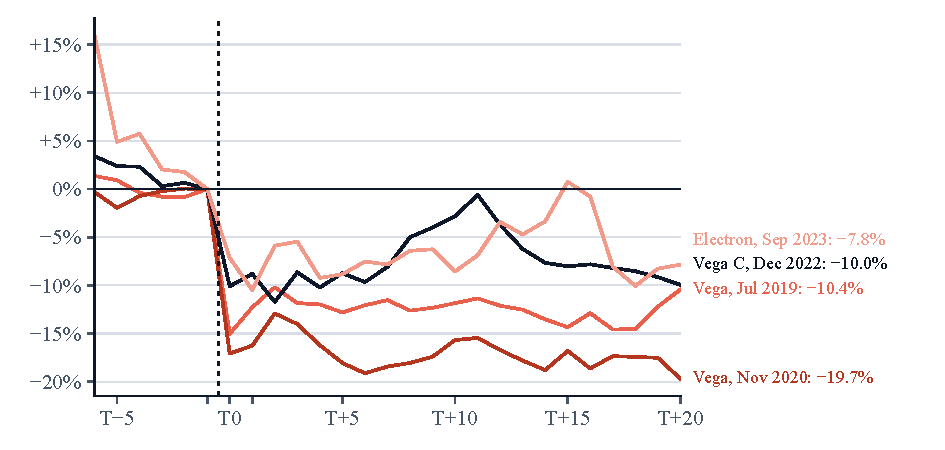
\includegraphics[width=\textwidth]{fig-paths.pdf}
\par\vspace{2pt}{\footnotesize Each line is one case, set to zero at the close before the failure (T\textminus{}1), so the value at T+1 is the two-day result in the table.}
\end{figure}

\subsection*{6.2 Listed competitors}
Table 4 reports the confirmatory test. The average two-day abnormal return of listed rivals is \textbf{+0.28\%} (95\% interval \textminus{}1.62\% to +2.18\%); the adjusted BMP statistic is 0.85 (p = 0.40). H2 is not rejected at the 5\% level.

\par\noindent\begin{minipage}{\textwidth}
\textbf{Table 4.} Confirmatory test of H2: listed competitors, CAR T0 to T+1

{\small\setlength{\tabcolsep}{4pt}\begin{tabularx}{\textwidth}{Xl}
\toprule
\textbf{Quantity} & \textbf{Value} \\
\midrule
Mean CAR, equal weight per reaction & +0.28\% \\
95\% cluster-robust interval (t, G\textminus{}1 df) & \textminus{}1.62\% to +2.18\% \\
Mean standardized CAR (BMP) & 0.227 \\
BMP t, unadjusted & 0.932 \\
Kolari-Pynnönen adjustment factor & 0.916 \\
Adjusted t / p (two-sided) & 0.854 / 0.40 \\
Mean within-cluster correlation & 0.150 \\
Reactions / failures / firms / clusters & 42 / 24 / 3 / 22 \\
Minimum detectable effect (80\% / 90\% power) & 2.7\% / 3.1\% \\
Power against a true ±1\% / ±2\% / ±3\% mean & 0.18 / 0.55 / 0.88 \\
90\% interval (for an equivalence reading) & \textminus{}1.29\% to +1.85\% \\
\bottomrule
\end{tabularx}}
\vspace{6pt}

Minimum detectable effect: two-sided 5\% test, from the cluster-robust standard error implied by the interval.

\end{minipage}\par\vspace{4pt}

\textbf{Precision.} With a cluster-robust standard error of 0.91\%, an average effect would need to be about 2.7\% to be detected with 80\% probability; the probability of detecting a true 1\% effect is 0.18. The 90\% interval (\textminus{}1.29\% to +1.85\%) would support an equivalence claim only for a margin of about ±1.9\%, which is not economically negligible for a two-day return. The data therefore do not show that rivals are unaffected.

\par\noindent\begin{minipage}{\textwidth}
\textbf{Table 5.} How the rival average depends on weighting

{\small\setlength{\tabcolsep}{4pt}\begin{tabularx}{\textwidth}{XlX}
\toprule
\textbf{Weighting} & \textbf{Estimate} & \textbf{Note} \\
\midrule
Every reaction equal (prespecified estimand) & +0.28\% & the main estimate \\
Every independent event equal & +0.21\% & same as the R1 portfolio average \\
Inverse prediction-error SD & +0.87\% & closest to the BMP statistic \\
Every firm equal & \textminus{}1.16\% & each firm's mean, then averaged \\
Median reaction & +0.28\% & not driven by a few large moves \\
\bottomrule
\end{tabularx}}
\vspace{6pt}

Descriptive, added after the audit; not new tests.

\end{minipage}\par\vspace{4pt}

The sign of the average depends on weighting: equal weight per reaction gives +0.28\%, equal weight per firm gives \textminus{}1.16\%, because Firefly Aerospace's 3 reactions average \textminus{}4.86\%. With 3 firms, asymptotic inference clustered by firm is not reliable, so firm-level dependence is examined by leaving each firm out (R8) rather than by clustering on firms.

\section*{7. Robustness and sensitivity}
None of the 12 prespecified checks detects a significant average at the 5\% level. Non-rejection is stable; the estimate is not: across checks the average ranges from \textminus{}0.15\% (Leave out AVIO.MI) to +1.84\% (Wider window, T\textminus{}1 to T+3). Leaving one firm out changes the sign.

\begin{figure}[htbp]\centering
\caption*{\textbf{Figure 5.} Listed competitors: main test and prespecified checks}
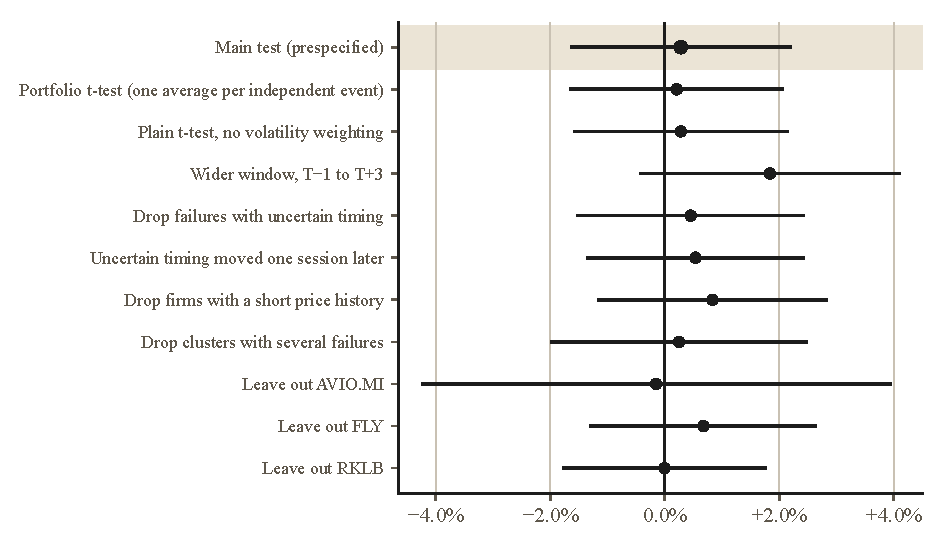
\includegraphics[width=\textwidth]{fig-forest.pdf}
\par\vspace{2pt}{\footnotesize Dots: average two-day abnormal return; lines: 95\% intervals. Shaded: the confirmatory test.}
\end{figure}

\par\noindent\begin{minipage}{\textwidth}
\textbf{Table 6.} Prespecified robustness checks

{\small\setlength{\tabcolsep}{4pt}\begin{tabularx}{\textwidth}{Xlllll}
\toprule
\textbf{Check} & \textbf{Average} & \textbf{95\% interval} & \textbf{p} & \textbf{Reactions} & \textbf{Clusters} \\
\midrule
Portfolio t-test (one average per independent event) & +0.21\% & \textminus{}1.63\% to +2.05\% & 0.82 & 42 & 22 \\
Sign test (share of events with a positive average) & +0.21\% & test only & 0.29 & 42 & 22 \\
Plain t-test, no volatility weighting & +0.28\% & \textminus{}1.57\% to +2.13\% & 0.76 & 42 & 22 \\
Rank test (simulated p-value) & +0.28\% & test only & 0.44 & 42 & 22 \\
Wider window, T\textminus{}1 to T+3 & +1.84\% & \textminus{}0.41\% to +4.09\% & 0.18 & 42 & 22 \\
Drop failures with uncertain timing & +0.45\% & \textminus{}1.52\% to +2.42\% & 0.37 & 40 & 21 \\
Uncertain timing moved one session later & +0.54\% & \textminus{}1.34\% to +2.41\% & 0.29 & 42 & 22 \\
Drop firms with a short price history & +0.83\% & \textminus{}1.15\% to +2.81\% & 0.27 & 38 & 21 \\
Drop clusters with several failures & +0.25\% & \textminus{}1.97\% to +2.47\% & 0.37 & 36 & 20 \\
Leave out AVIO.MI & \textminus{}0.15\% & \textminus{}4.23\% to +3.93\% & 0.77 & 18 & 14 \\
Leave out FLY & +0.68\% & \textminus{}1.28\% to +2.63\% & 0.30 & 39 & 22 \\
Leave out RKLB & 0.00\% & \textminus{}1.76\% to +1.75\% & 0.52 & 27 & 22 \\
\bottomrule
\end{tabularx}}
\vspace{6pt}

\end{minipage}\par\vspace{4pt}

\textbf{Placebo.} R9 repeats the calculation on 1000 sets of random ordinary trading days. The real result sits at the 61st percentile (two-sided share 0.776). Because R9 draws a separate date for each reaction, it ignores that rivals hit by one failure move on the same day, so its spread is too narrow; it is a benchmark, not an exact permutation test, and the percentile is not a probability that the effect is real. An exploratory version with one shared date per cluster (R9b, 1000 draws) places the real result at the 66th percentile (two-sided share 0.684).

\begin{figure}[htbp]\centering
\caption*{\textbf{Figure 6.} Real result against random ordinary days (R9)}
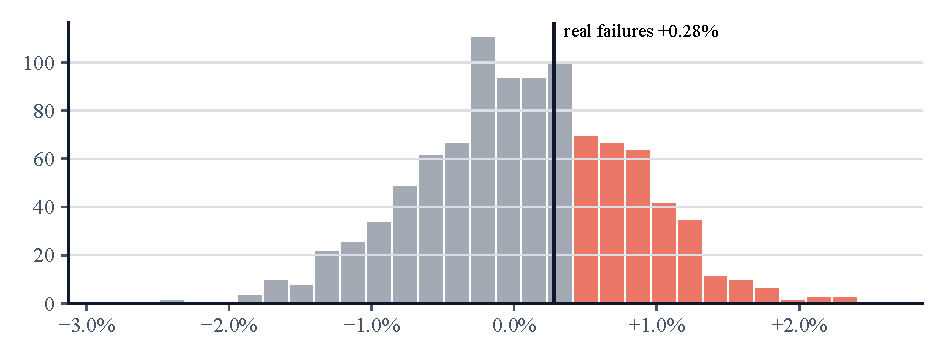
\includegraphics[width=\textwidth]{fig-placebo.pdf}
\par\vspace{2pt}{\footnotesize Histogram of 1000 placebo averages (fixed seed). Red: averages at least as far out as the real result. Black line: the real failures.}
\end{figure}

\section*{8. Confounding news}
An event study attributes every unusual return in the window to the event. If a firm announces something else on the same days, its reaction mixes the two. The news around the largest rival reactions was therefore checked against public sources. Flagged reactions stay in the confirmatory test, because the plan does not allow removing events after results are seen.

\par\noindent\begin{minipage}{\textwidth}
\textbf{Table 7.} Rival reactions with other news in the window

{\small\setlength{\tabcolsep}{4pt}\begin{tabularx}{\textwidth}{lXllX}
\toprule
\textbf{Firm} & \textbf{Failure} & \textbf{CAR} & \textbf{Verdict} & \textbf{News} \\
\midrule
Rocket Lab & Firefly Alpha, 22 Dec 2023 & +25.27\% & confounded & USD 515m Space Development Agency contract announced in the same window \href{https://www.fool.com/investing/2023/12/22/why-rocket-lab-stock-is-going-to-the-moon-today}{[source]} \\
Avio SpA & Kairos, 18 Dec 2024 & +14.51\% & confounded & EUR 350m ESA contracts released 18 Dec 2024 after the Milan close (day +1) \href{https://www.emarketstorage.it/sites/default/files/comunicati/2024-12/20241218_158732.pdf}{[source]} \\
Firefly Aerospace & PSLV-DL, 12 Jan 2026 & \textminus{}6.98\% & possibly confounded & Securities class-action lead-plaintiff deadline on day 0 \href{https://finviz.com/news/268191/shareholders-of-firefly-aerospace-inc-should-contact-levi-korsinsky-before-january-12-2026-to-discuss-your-rights-fly}{[source]} \\
Rocket Lab & Spectrum, 31 Mar 2025 & \textminus{}6.49\% & sector move & Broad tech and space-stock selloff on day 0 not absorbed by the S\&P 500 benchmark \href{https://finviz.com/news/13588/why-rocket-lab-planet-labs-and-ast-spacemobile-stocks-all-dropped-on-monday}{[source]} \\
\bottomrule
\end{tabularx}}
\vspace{6pt}

\end{minipage}\par\vspace{4pt}

The exploratory specifications below drop the flagged reactions. Dropping the 2 contract-news days changes the average from +0.28\% to \textminus{}0.70\%, but the median moves only from +0.28\% to +0.09\%: the change comes from removing two large positive moves, not from a shift in the typical reaction. The standardized test barely moves (p = 0.86), because it gives less weight to the volatile stocks behind those moves. The exploratory estimates are not more correct than the prespecified one: the choice of what to drop was made after seeing the data.

\par\noindent\begin{minipage}{\textwidth}
\textbf{Table 8.} Confounding-news sensitivity (exploratory)

{\small\setlength{\tabcolsep}{4pt}\begin{tabularx}{\textwidth}{Xllllll}
\toprule
\textbf{Specification} & \textbf{Average} & \textbf{95\% interval} & \textbf{p} & \textbf{Median} & \textbf{Reactions} & \textbf{Clusters} \\
\midrule
Main test (prespecified) & +0.28\% & \textminus{}1.62\% to +2.18\% & 0.40 & +0.28\% & 42 & 22 \\
Drop the contract-news days (exploratory) & \textminus{}0.70\% & \textminus{}1.80\% to +0.39\% & 0.86 & +0.09\% & 40 & 22 \\
Also drop possible same-day news (exploratory) & \textminus{}0.54\% & \textminus{}1.71\% to +0.63\% & 0.95 & +0.26\% & 39 & 22 \\
Drop every flagged day (exploratory) & \textminus{}0.38\% & \textminus{}1.58\% to +0.82\% & 0.95 & +0.28\% & 38 & 22 \\
\bottomrule
\end{tabularx}}
\vspace{6pt}

\end{minipage}\par\vspace{4pt}

\begin{figure}[htbp]\centering
\caption*{\textbf{Figure 7.} Confounding-news sensitivity}
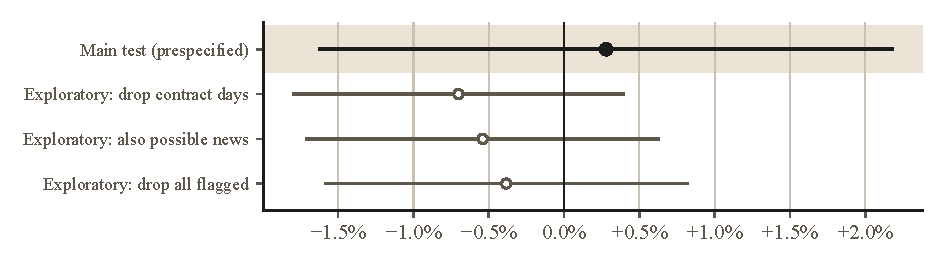
\includegraphics[width=\textwidth]{fig-conf.pdf}
\par\vspace{2pt}{\footnotesize Shaded: the confirmatory test. Hollow: exploratory specifications that drop flagged reactions.}
\end{figure}

\section*{9. Discussion}
The evidence supports two statements. First, listed makers lose substantial value when their rocket fails, in a small set of cases. Second, the average reaction of listed rivals cannot be distinguished from zero in this sample.

Several mechanisms are consistent with a small net rival reaction: contagion and competitive gain may both be present and offset each other; customers may be unable to switch quickly because contracts and satellites are tied to particular rockets; or investors may treat failures mainly as news about the failed firm. None of these mechanisms is identified here. Distinguishing them would require customer-level data on contract moves, launch backlogs, or a much larger sample of listed rivals. The results also say nothing about private, state-owned or diversified aerospace firms.

\section*{10. Limitations}
\begin{itemize}[leftmargin=*,itemsep=2pt,topsep=4pt]
  \item \textbf{Few listed firms.} 3 rival firms and 22 independent events; Avio SpA appears in all of them. Repeated exposure of the same stock means clustering by event captures only part of the dependence.
  \item \textbf{Power.} Average effects of about 2.7\% could go undetected; no equivalence claim is possible.
  \item \textbf{Weighting and outliers.} The sign of the estimate depends on weighting and on two large reactions with contract news.
  \item \textbf{Two estimands.} The interval (equal-weighted mean) and the test (standardized mean) concern different quantities and can disagree.
  \item \textbf{Timing.} A few failures are dated by later company statements; one of these is uncertain. R5 checks cover them.
  \item \textbf{Model dependence.} A one-factor market model with a home index; sector-wide moves on event days are not absorbed (one flagged case).
  \item \textbf{Survivorship.} Listed launch firms that later delisted (Orbital Sciences/Orbital ATK, Astra, Virgin Orbit) are missing because the free price source does not carry them.
  \item \textbf{External validity.} The population is historically eligible, publicly traded launch-service competitors with comparable commercial exposure, not the launch industry.
  \item \textbf{Data quality.} Yahoo adjusted prices and GCAT records are good but not audited sources; price-quality issues are logged in the pipeline.
  \item \textbf{Prespecification.} The plan was committed to git before results but not filed with an independent registry; git timestamps are set by the author.
\end{itemize}

\section*{11. Conclusion}
When an orbital rocket fails, its listed maker loses a large share of its value within two days in every case observed. For listed competitors, the average two-day reaction is +0.28\%, with an interval from \textminus{}1.62\% to +2.18\%. The data do not establish contagion or competitive gains, and they do not rule out either at magnitudes of a few percent. The study is useful as a transparent, reproducible baseline: every number can be recomputed from the published data, and adding more listed firms, including delisted ones and SpaceX as its price history grows, would sharpen the answer without changing the prespecified test.

\section*{References}
\begin{enumerate}[leftmargin=*,itemsep=2pt,topsep=4pt]
  \item Abramov, D. and Kiang, C. (2015). Effect of space launch delays and failures on stock market returns of commercial payload operators. International Astronautical Congress, IAC-15,E6,1,1,x29453.
  \item Blose, L. E., Bornkamp, R., Brier, M., Brown, K. and Frederick, J. (1996). Catastrophic events, contagion, and stock market efficiency: the case of the space shuttle Challenger. \emph{Review of Financial Economics} 5(2), 117-129.
  \item Boehmer, E., Musumeci, J. and Poulsen, A. B. (1991). Event-study methodology under conditions of event-induced variance. \emph{Journal of Financial Economics} 30(2), 253-272.
  \item Bosch, J.-C., Eckard, E. W. and Singal, V. (1998). The competitive impact of air crashes: stock market evidence. \emph{Journal of Law and Economics} 41(2), 503-519.
  \item Brown, S. J. and Warner, J. B. (1985). Using daily stock returns: the case of event studies. \emph{Journal of Financial Economics} 14(1), 3-31.
  \item Campbell, J. Y., Lo, A. W. and MacKinlay, A. C. (1997). \emph{The Econometrics of Financial Markets}. Princeton University Press.
  \item Corrado, C. J. (1989). A nonparametric test for abnormal security-price performance in event studies. \emph{Journal of Financial Economics} 23(2), 385-395.
  \item Do, H. X., Nguyen, N. H., Nguyen, Q. M. P. and Truong, C. (2023). Aerospace competition, investor attention, and stock return comovement. \emph{Journal of Economic Behavior \& Organization} 215, 40-59.
  \item Kaplanski, G. and Levy, H. (2010). Sentiment and stock prices: the case of aviation disasters. \emph{Journal of Financial Economics} 95(2), 174-201.
  \item Kolari, J. W. and Pynnönen, S. (2010). Event study testing with cross-sectional correlation of abnormal returns. \emph{Review of Financial Studies} 23(11), 3996-4025.
  \item Lang, L. H. P. and Stulz, R. M. (1992). Contagion and competitive intra-industry effects of bankruptcy announcements. \emph{Journal of Financial Economics} 32(1), 45-60.
  \item MacKinlay, A. C. (1997). Event studies in economics and finance. \emph{Journal of Economic Literature} 35(1), 13-39.
  \item Maloney, M. T. and Mulherin, J. H. (2003). The complexity of price discovery in an efficient market: the stock market reaction to the Challenger crash. \emph{Journal of Corporate Finance} 9(4), 453-479.
  \item McDowell, J. C. GCAT: General Catalog of Artificial Space Objects. planet4589.org/space/gcat.
\end{enumerate}

\section*{Appendix A. Rival event list}
\textbf{Table 9.} All rival reactions, CAR T0 to T+1

{\scriptsize\setlength{\tabcolsep}{4pt}\begin{xltabular}{\textwidth}{lllllllXll}
\toprule
\textbf{Failure} & \textbf{Rocket} & \textbf{T0} & \textbf{Ticker} & \textbf{Cluster} & \textbf{Model} & \textbf{Timing} & \textbf{Flag} & \textbf{CAR} & \textbf{SD} \\
\midrule
\endhead
2017-051 & PSLV-XL & 2017-08-31 & AVIO.MI & 58 & MA & high &  & \textminus{}0.86\% & 2.21\% \\
2020-F04 & LauncherOne & 2020-05-26 & AVIO.MI & 74 & MM & provisional &  & \textminus{}3.08\% & 2.73\% \\
2020-F05 & Electron & 2020-07-06 & AVIO.MI & 75 & MM & provisional &  & \textminus{}0.09\% & 2.88\% \\
2020-F07 & Astra Rocket 3.1 & 2020-09-14 & AVIO.MI & 76 & MM & provisional &  & \textminus{}4.32\% & 2.68\% \\
2020-F09 & Astra Rocket 3.2 & 2020-12-16 & AVIO.MI & 77 & MM & provisional &  & +2.99\% & 2.87\% \\
2021-F02 & Electron & 2021-05-17 & AVIO.MI & 81 & MM & provisional &  & +1.30\% & 3.02\% \\
2021-F07 & Astra Rocket 3.3 & 2021-08-30 & AVIO.MI & 84 & MM & provisional &  & +1.59\% & 3.26\% \\
2021-F08 & Firefly Alpha & 2021-09-03 & AVIO.MI & 84 & MM & provisional &  & \textminus{}3.77\% & 3.25\% \\
2022-F01 & Astra Rocket 3.3 & 2022-02-10 & RKLB & 87 & MA & high &  & \textminus{}6.00\% & 9.37\% \\
2022-F01 & Astra Rocket 3.3 & 2022-02-11 & AVIO.MI & 87 & MM & high &  & +0.26\% & 2.44\% \\
2022-F03 & Astra Rocket 3.3 & 2022-06-13 & AVIO.MI & 89 & MM & provisional &  & \textminus{}7.25\% & 2.82\% \\
2022-F03 & Astra Rocket 3.3 & 2022-06-13 & RKLB & 89 & MM & provisional &  & +0.43\% & 7.91\% \\
2023-F01 & LauncherOne & 2023-01-10 & AVIO.MI & 94 & MM & provisional &  & \textminus{}3.93\% & 3.64\% \\
2023-F01 & LauncherOne & 2023-01-10 & RKLB & 94 & MM & provisional &  & +3.31\% & 5.48\% \\
2023-F02 & RS1 & 2023-01-11 & AVIO.MI & 94 & MM & provisional &  & \textminus{}1.78\% & 3.65\% \\
2023-F02 & RS1 & 2023-01-11 & RKLB & 94 & MM & provisional &  & +7.33\% & 5.48\% \\
2023-F04 & Terran 1 & 2023-03-23 & AVIO.MI & 95 & MM & provisional &  & \textminus{}0.93\% & 3.42\% \\
2023-F04 & Terran 1 & 2023-03-23 & RKLB & 95 & MM & provisional &  & +0.72\% & 5.26\% \\
2023-F08 & Electron & 2023-09-19 & AVIO.MI & 98 & MM & provisional &  & \textminus{}0.56\% & 2.38\% \\
2023-202 & Firefly Alpha & 2023-12-22 & RKLB & 93 & MM & provisional & confounded & +25.27\% & 4.67\% \\
2023-202 & Firefly Alpha & 2023-12-27 & AVIO.MI & 93 & MM & provisional &  & +6.35\% & 1.84\% \\
2024-F01 & Kairos & 2024-03-13 & AVIO.MI & 100 & MM & provisional &  & +4.65\% & 1.75\% \\
2024-F01 & Kairos & 2024-03-13 & RKLB & 100 & MM & provisional &  & \textminus{}2.78\% & 5.05\% \\
2024-F04 & Kairos & 2024-12-18 & AVIO.MI & 103 & MM & provisional & confounded & +14.51\% & 2.65\% \\
2024-F04 & Kairos & 2024-12-18 & RKLB & 103 & MM & provisional &  & \textminus{}7.31\% & 5.99\% \\
2025-F04 & Spectrum & 2025-03-31 & AVIO.MI & 106 & MM & provisional &  & +2.69\% & 2.81\% \\
2025-F04 & Spectrum & 2025-03-31 & RKLB & 106 & MM & provisional & sector move & \textminus{}6.49\% & 6.99\% \\
2025-U01 & Firefly Alpha & 2025-04-29 & AVIO.MI & 111 & MM & low &  & +1.12\% & 3.00\% \\
2025-U01 & Firefly Alpha & 2025-04-29 & RKLB & 111 & MM & low &  & \textminus{}7.45\% & 7.15\% \\
2025-F05 & PSLV-XL & 2025-05-19 & AVIO.MI & 107 & MM & provisional &  & +3.37\% & 3.10\% \\
2025-F05 & PSLV-XL & 2025-05-19 & RKLB & 107 & MM & provisional &  & +0.85\% & 7.15\% \\
2025-F06 & Eris Block 1 & 2025-07-30 & AVIO.MI & 108 & MM & provisional &  & +0.41\% & 3.60\% \\
2025-F06 & Eris Block 1 & 2025-07-30 & RKLB & 108 & MM & provisional &  & +4.54\% & 7.40\% \\
2025-F09 & HANBIT-NANO & 2025-12-23 & AVIO.MI & 113 & MM & provisional &  & \textminus{}1.50\% & 5.50\% \\
2025-F09 & HANBIT-NANO & 2025-12-23 & FLY & 113 & MA & provisional &  & \textminus{}6.07\% & 7.54\% \\
2025-F09 & HANBIT-NANO & 2025-12-23 & RKLB & 113 & MM & provisional &  & \textminus{}2.83\% & 6.83\% \\
2026-F01 & PSLV-DL & 2026-01-12 & AVIO.MI & 115 & MM & provisional &  & +3.00\% & 5.58\% \\
2026-F01 & PSLV-DL & 2026-01-12 & FLY & 115 & MA & provisional & possibly confounded & \textminus{}6.98\% & 8.26\% \\
2026-F01 & PSLV-DL & 2026-01-12 & RKLB & 115 & MM & provisional &  & +1.83\% & 6.75\% \\
2026-F04 & Kairos & 2026-03-05 & AVIO.MI & 116 & MM & provisional &  & +0.30\% & 5.71\% \\
2026-F04 & Kairos & 2026-03-05 & FLY & 116 & MM & provisional &  & \textminus{}1.53\% & 9.37\% \\
2026-F04 & Kairos & 2026-03-05 & RKLB & 116 & MM & provisional &  & +0.43\% & 6.51\% \\
\bottomrule
\end{xltabular}}
\vspace{6pt}

Model: MM market model, MA market-adjusted fallback. SD: prediction-error standard deviation of the CAR.

\section*{Appendix B. Firm mapping and rival criteria}
Rivals are classified point in time from the hand-built firm map (\texttt{data/manual/firm\_map.csv}) and the size-and-market table (\texttt{data/manual/vehicle\_segments.csv}): listing dates, ownership, exposure and sources are recorded per row. Tier 1 requires the same size class and customer market, launch as a pure-play or major business, and a flight in the prior 730 days. Diversified aerospace groups are classified as minor exposure and enter only descriptive tiers.

\section*{Appendix C. Additional exploratory results}
\par\noindent\begin{minipage}{\textwidth}
\textbf{Table 10.} Exploratory comparisons (Holm-adjusted p-values)

{\small\setlength{\tabcolsep}{4pt}\begin{tabularx}{\textwidth}{Xlll}
\toprule
\textbf{Comparison} & \textbf{Estimate} & \textbf{p} & \textbf{p (Holm)} \\
\midrule
Competitors: first-flight failures minus other failures & \textminus{}1.33\% & 0.45 & 0.89 \\
Maker: failures minus successful launches & \textminus{}11.84\% & 0.002 & 0.005 \\
Competitors over one month (T0 to T+20) & +0.83\% & 0.72 & 0.89 \\
\bottomrule
\end{tabularx}}
\vspace{6pt}

\end{minipage}\par\vspace{4pt}

\section*{Appendix D. Statistical verification}
An independent script (\texttt{audit/verify\_published.py}) recomputes the published statistics from the published derived data without importing the pipeline; 81 of 81 quantities reproduce within tolerance (1e-9 for estimates and intervals, 1e-8 for t and p). The CARs themselves need licensed prices and are reproduced by re-running the pipeline.

\section*{Appendix E. Exclusions}
\par\noindent\begin{minipage}{\textwidth}
\textbf{Table 11.} Failures not in the study, by reason

{\small\setlength{\tabcolsep}{4pt}\begin{tabularx}{\textwidth}{Xl}
\toprule
\textbf{Reason} & \textbf{Failures} \\
\midrule
maker not a listed company & 97 \\
no listed maker or listed competitor & 13 \\
maker not listed, or not the owner, on that date & 1 \\
\bottomrule
\end{tabularx}}
\vspace{6pt}

A failure can have more than one reason, so the counts can add up to more than the number of excluded failures.

\end{minipage}\par\vspace{4pt}

\section*{Appendix F. Reproduction guide}
\begin{enumerate}[leftmargin=*,itemsep=2pt,topsep=4pt]
  \item Install Python 3.11+ and \texttt{pip install -r requirements.txt}.
  \item \texttt{python pipeline/01\_ingest\_launches.py} downloads GCAT and classifies launches; \texttt{02\_map\_firms.py} applies the firm map.
  \item \texttt{03\_pull\_prices.py} downloads prices (Yahoo Finance; not redistributed); \texttt{04\_check\_coverage.py} writes the feasibility gate.
  \item \texttt{05\_event\_study.py} runs the prespecified analysis; \texttt{06} and \texttt{09} run the exploratory checks.
  \item \texttt{07\_export\_site\_data.py} exports derived statistics; \texttt{08\_build\_html.py} builds the site and this paper; \texttt{python audit/verify\_published.py} re-checks every statistic.
  \item \texttt{python -m pytest tests} runs the test suite.
\end{enumerate}

\section*{Where to find the charts, data and code}
{\small\setlength{\tabcolsep}{4pt}\begin{tabularx}{\textwidth}{XX}
\toprule
\textbf{Resource} & \textbf{What it is} \\
\midrule
\href{https://nahianibnat-2000.github.io/T-Minus-Market/index.html}{The article (one-page summary)} & Key numbers and links \\
\href{https://nahianibnat-2000.github.io/T-Minus-Market/site/index.html}{Interactive report} & Five stages and four interactive tools \\
\href{https://nahianibnat-2000.github.io/T-Minus-Market/plan.html}{Analysis plan and change log} & Rules fixed before results, and every later change \\
\href{https://github.com/NahianIbnat-2000/T-Minus-Market/blob/master/reports/04_feasibility_report.md}{Feasibility report} & Sample and minimum detectable effects, before results \\
\href{https://github.com/NahianIbnat-2000/T-Minus-Market/blob/master/reports/05_results.md}{Results report} & All prespecified results \\
\href{https://github.com/NahianIbnat-2000/T-Minus-Market/blob/master/docs/CONFOUNDING_NEWS.md}{Confounding-news checks} & News around the largest reactions, with sources \\
\href{https://github.com/NahianIbnat-2000/T-Minus-Market/blob/master/audit/AUDIT_REPORT.md}{Independent audit} & Verification of every published statistic \\
\href{https://github.com/NahianIbnat-2000/T-Minus-Market}{Code and pipeline} & Python pipeline, tests and reproduction guide \\
 &  \\
\bottomrule
\end{tabularx}}
\vspace{6pt}

\vspace{1.5em}\noindent\rule{\textwidth}{0.4pt}\par\noindent{\small Nahian Ibnat, Nov 2026. Cite as: Ibnat, N. (2026). \emph{Rocket Launch Failures and Equity-Market Spillovers: Evidence from Publicly Listed Launch Providers.} T-Minus Markets working paper. https://nahianibnat-2000.github.io/T-Minus-Market/case-study.html Research, not investment advice. \href{https://nahianibnat-2000.github.io/}{Portfolio} \textperiodcentered{} \href{https://www.linkedin.com/in/nahian-ibnat}{LinkedIn}}

\end{document}
